% Этот текст можно свободно редактировать.
\FloatBarrier
\section{Результат и исследовательский вопрос}

Можно ли автоматически подобрать временные окна и отношения между сущностями так, чтобы улучшить сильный CatBoost с ручными признаками? Проверяется ограниченный, интерпретируемый поиск по грамматике агрегатов. Это исследование автоматизации признаков, а не новой архитектуры нейросети.

Ручной baseline: \textbf{NDCG@10 = 0.47332}. Автоотбор: \textbf{0.48440}. Разница \textbf{+0.01107} (+2.34\% относительно baseline), 95\% ДИ \textbf{[+0.00840, +0.01383]}. Автоматический отбор улучшил основную метрику, и парный 95\% интервал не включает ноль. Вывод относится к оговорённому офлайн-протоколу и выбранной выборке.

Два существенных ограничения исходного результата: \textbf{весь банк без отбора дал 0.49114 при seed 42}, обойдя выбранное подмножество; \textbf{на полном каталоге популярность за 7 дней получила 0.14847, автоотбор --- 0.10332}. Повторения банка и проверка причины потерь отбора добавлены в §10. На полном каталоге положительная разность статистически не подтверждена: интервал включает ноль. Поэтому подтверждён вывод об улучшении заданной задачи переранжирования, а не о готовой замене популярности в поиске по всему каталогу.

\begin{figure}[!htbp]
\centering
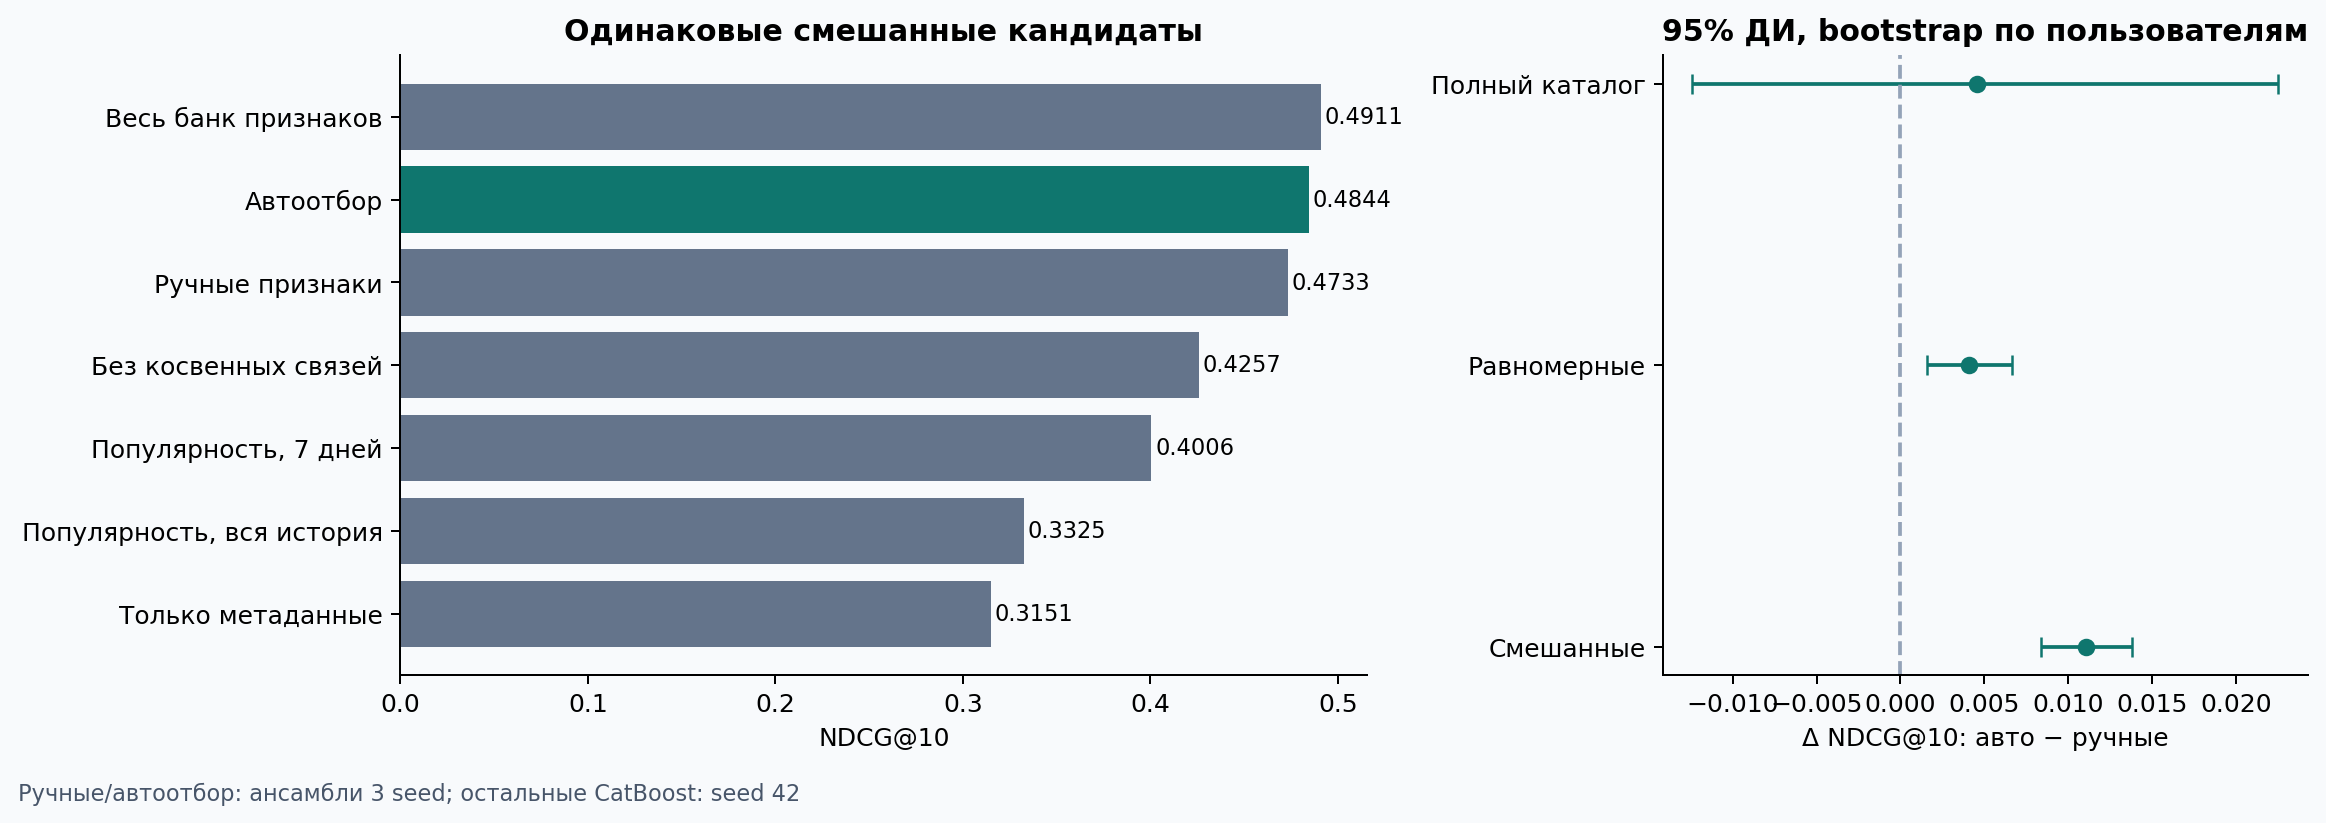
\includegraphics[width=\linewidth,height=.70\textheight,keepaspectratio]{figures/results.png}
\caption{Результаты и доверительные интервалы}
\label{fig:results}
\end{figure}
